\subsection{Constant-leaf forests}
\label{sec:constant}
Constant predictions simplify the hardware leaf stage and permit comparison
with scalar-leaf FPGA tree architectures~\cite{conifer2020}. To study the
accuracy cost, we scan $T\in\{1,3,5\}$ trees, $D\in\{2,3,4\}$ and
$\lambda_s\in\{0,10^{-7},10^{-5}\}$, giving 27 configurations. Each uses the
same CART initialization seed, training partition and numerical stopping rules
as the factorial architecture study. Constant leaves have no feature weights,
so their nominal leaf penalty does not affect Eq.~\eqref{eq:objective}.
We select the saved checkpoint with the highest validation efficiency at
1\% background from each converged source run, and then select among
penalties for each layout.

\ifnum\ConstantCompleted<\ConstantTotal\relax
At this snapshot, \ConstantCompleted{} of \ConstantTotal{} source runs have
converged. The remaining five-tree, depth-four run with $\lambda_s=10^{-7}$
is still training and contributes no selected result. Table~\ref{tab:constant}
therefore reports the best eligible completed case per layout.
\else
All \ConstantTotal{} source runs have converged.
Table~\ref{tab:constant} reports the best selected penalty per layout.
\fi
The interpolated efficiency follows the common ROC convention. We also report
a strict threshold on the binary64 signal margin that accepts at most 525
background events. This distinction matters for shallow constant trees:
a single depth-$D$ tree has at most $2^D$ score levels, and even its highest
level can exceed the background budget. Connecting ROC vertices then gives
an interpolated efficiency that a deterministic threshold cannot realize.

\begin{table}[htbp]\centering\small
\caption{Constant-leaf forests: the best eligible penalty per layout.
$\epsilon_s$ is interpolated at 1\% background; $\epsilon_s^{\rm strict}$ uses
a realizable strict margin threshold with background efficiency at most 1\%.
Both coefficient counts include biases.}
\label{tab:constant}\setlength{\tabcolsep}{4pt}
\begin{tabular}{@{}lrrrrrr@{}}\toprule
Layout & $\lambda_s$ & $P_{\rm dense}$ & $P_{\rm nz}$ & $\epsilon_s$ [\%] & $\epsilon_s^{\rm strict}$ [\%] & AUC\\\midrule
1 $\times$ D2 & $10^{-7}$ & 55 & 55 & 14.98 & 0.00 & 0.88179 \\
1 $\times$ D3 & $10^{-5}$ & 127 & 126 & 38.61 & 0.00 & 0.90357 \\
1 $\times$ D4 & 0 & 271 & 256 & 45.36 & 45.33 & 0.91247 \\
3 $\times$ D2 & $10^{-5}$ & 165 & 129 & 30.72 & 0.00 & 0.90087 \\
3 $\times$ D3 & 0 & 381 & 336 & 49.01 & 38.81 & 0.91763 \\
3 $\times$ D4 & 0 & 813 & 753 & 53.54 & 53.30 & 0.92318 \\
5 $\times$ D2 & $10^{-7}$ & 275 & 275 & 47.77 & 47.01 & 0.91283 \\
5 $\times$ D3 & $10^{-7}$ & 635 & 615 & 50.94 & 50.31 & 0.92176 \\
5 $\times$ D4 & 0 & 1355 & 1250 & 55.40 & 54.75 & 0.92610 \\
\bottomrule
\end{tabular}
\end{table}

The selected constant configuration has \ConstantWinnerTrees{} trees of
depth \ConstantWinnerDepth{}, with \ConstantWinnerNonzero{} nonzeros in
\ConstantWinnerDense{} allocated slots. It reaches
\ConstantWinnerEfficiency\% interpolated signal efficiency; its realizable
strict-threshold efficiency is \ConstantWinnerStrict\%.
Figure~\ref{fig:constant} compares the depth-four constant forests with XGBoost
and the sparse linear-leaf Compact refit. These are comparisons of selected
configurations: their penalty and refitting histories differ, so the comparison
is not a leaf-type ablation at identical support.
\begin{figure}[htbp]\centering
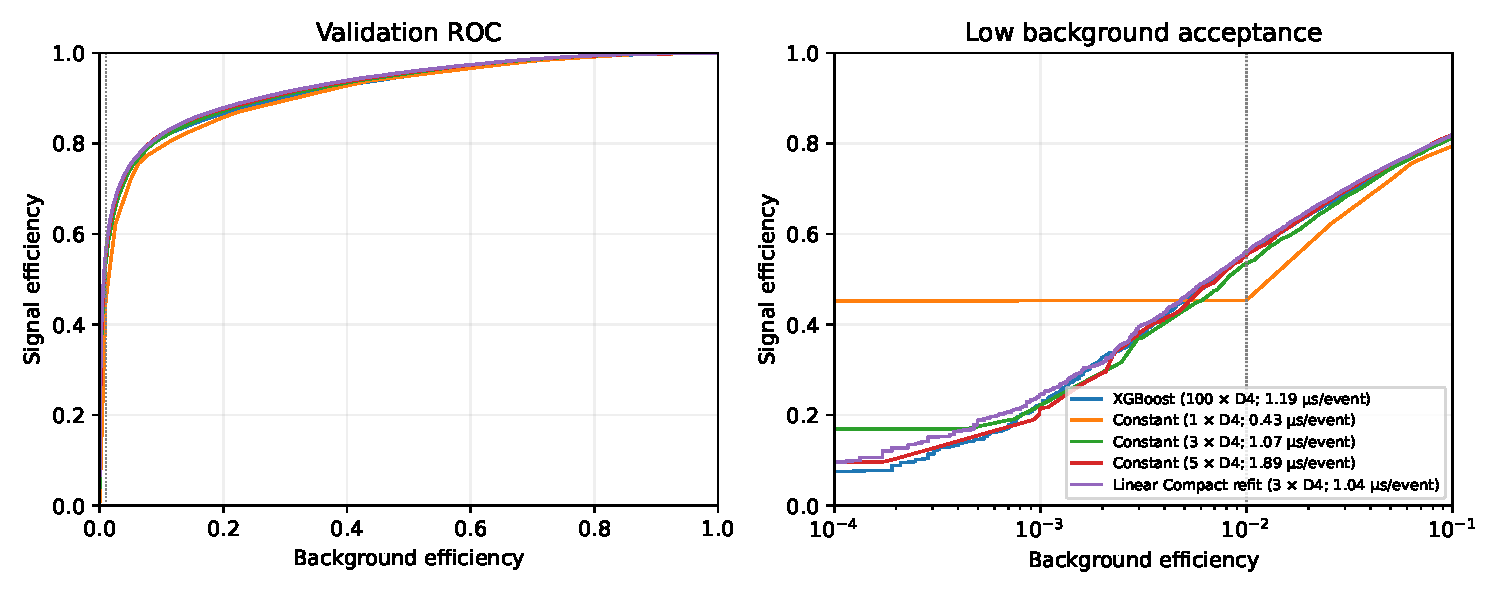
\includegraphics[width=\textwidth]{figures/constant_leaf_roc.pdf}
\caption{Validation ROCs for the best completed constant-leaf configuration at
each depth-four layout, compared with XGBoost and linear-leaf Compact refit.
The low-background panel exposes the coarse score steps of small constant
forests. Eligibility requires convergence of the source run; selection can
choose an earlier saved epoch. Parenthetical times are bulk CPU wall time per
event on the 132,800-event batch: one thread, median of nine repeats. TAO uses
the NumPy prediction API on binary64 inputs and XGBoost uncached compiled
prediction on preconverted binary32 inputs. These follow-up measurements are separate from Table~\ref{tab:main}
and are not FPGA or single-event latency.}
\label{fig:constant}
\end{figure}
\FloatBarrier

For these candidates, linear predictions reduce the number of nonzero
coefficients from 1250 to 418, a factor of 2.99, while increasing the
interpolated signal efficiency from 55.40\% to 56.20\%.
After eliminating only input-independent branches and exact-zero terms,
the respective all-node multiplication counts are 1095 and 327; selected-path
upper bounds are 275 and 80. The additional leaf arithmetic is therefore
more than offset by the sparser, smaller forest in this comparison.
These scalar operation counts do not determine synthesized resource use:
precision, scheduling, constant-multiplier optimization and storage layout
must also be specified.




A matched compiled sparse traversal provides an additional CPU check. With
one thread and the full 132,800-event validation batch, the median of nine
repeats after one warmup is \LeafConstantCPU{} microseconds per event for
the constant forest and \LeafLinearCPU{} for the linear forest.
Both use binary64 arithmetic and the same traversal strategy; input conversion
and file I/O are excluded. These are CPU batch measurements, with no inference
about FPGA latency.

For an exploratory reduced-precision comparison, each cut is first multiplied
by a positive power of two, $w'_{tv}=2^{k_{tv}}w_{tv}$ and
$b'_{tv}=2^{k_{tv}}b_{tv}$. This preserves its real-arithmetic decision; the
exported binary64 scaling is constrained to retain every nonzero coefficient,
and validation leaf assignments are checked before quantization.
We use the nearest-even, saturating quantizer of Eq.~\eqref{eq:quantizer}, with
10 integer bits for inputs, thresholds and cut accumulators, 6 for weights,
and 16 for scores and leaf biases, all including sign. Every type uses the
same fractional width $F$. Cast inputs and coefficients precede multiplication;
cut products accumulate in feature order, with a cast to the cut-accumulator
format after each addition. For a linear leaf, products accumulate similarly
in the score format, followed by the leaf bias. The negative tree outputs are
summed in the score format. Integer widths are conservatively checked against
absolute partial-sum bounds in the observed training box; they have not been
minimized separately for the two candidates.

\begin{table}[htbp]\centering\small
\caption{Common-format fixed-point emulation of the two selected leaf
architectures. Efficiencies are percentages at 1\% background. Total widths
are $F+10$ input/threshold bits, $F+6$ weight bits and $F+16$ score bits.}
\label{tab:leafprecision}
\begin{tabular}{@{}lrrr@{}}\toprule
Leaf type & $F$ & $\epsilon_s$ [\%] & $\epsilon_s^{\rm strict}$ [\%]\\\midrule
Constant & 18 & 55.40 & 54.75 \\
Constant & 12 & 55.40 & 54.75 \\
Constant & 8 & 55.18 & 54.38 \\
Linear & 18 & 56.20 & 56.20 \\
Linear & 12 & 56.21 & 56.21 \\
Linear & 8 & 56.00 & 56.00 \\
\bottomrule
\end{tabular}
\end{table}
At $F=12$, both architectures remain within 0.02 percentage points of their
floating-point interpolated working-point efficiency (Table~\ref{tab:leafprecision}).
For constant leaves, independent fixed-point path traversal and the existing
weighted-cut backend agree exactly on all validation scores. The generated
all-node HLS C++ implementation also agrees exactly on a 512-vector check at
$F=12$. The linear-leaf evaluation uses an independent affine-leaf reference;
a corresponding HLS backend extension and synthesis remain to be completed.
These checks establish numerical feasibility at common precision, rather than
an optimized FPGA resource comparison.

\begin{implementation}
\textbf{Controlled cohort and exact snapshots.}
The constant subset of \file{configs/tao_hyper_scan_v1.json} comprises cases
3--5, 9--11, 15--17, 21--23, 27--29, 33--35, 39--41, 45--47 and 51--53.
These use CART initialization and hard-threshold search. They are separate
from the earlier seven-layout, randomly initialized constant study.
\file{scripts/build_constant_leaf_study.py} re-evaluates eligible checkpoints,
archives them under \code{models/constant_study_v1_selected/<sha256>.pkl},
and records selected and terminal epochs, metrics, configurations, convergence
checks and hashes in \code{paper/sources/constant_leaf_study.json}.
The selected constant model is also exported in
\code{paper/sources/constant_leaf_winner.json}; this does not alter the v3
handover or its default. Its selected epoch is \ConstantWinnerEpoch{}, while
the source run terminates at epoch \ConstantWinnerTerminalEpoch{}.

Regenerate with the pinned training environment:
\begin{lstlisting}[language=bash]
PYTHONPATH=src:. python scripts/build_constant_leaf_study.py
# Final gate: exits unsuccessfully while any source case is incomplete.
PYTHONPATH=src:. python scripts/build_constant_leaf_study.py --require-complete
\end{lstlisting}
The two-candidate entry point is
\file{fpga_handoff/CURRENT_CANDIDATES.json}. The constant winner is frozen in
\code{fpga_handoff/leaf_competition_v1/constant_5t_d4/}; the linear candidate
points to the unchanged v3 Compact refit. Both input spaces have canonical
JSON, hexadecimal coefficients and golden vectors.
\file{docs/leaf_competition_v1/README.md} records CPU/precision results and
\file{scripts/run_leaf_competition.sh} reproduces them in the pinned EL9
container. The scalar-leaf adapter uses unmodified conifer 1.11; the CMSSW
1.7 external cannot evaluate oblique weights. The affine-leaf reference is
\file{fpga/leaf_competition/emulate.cc}, not a conifer HLS backend extension.
\file{scripts/verify_fpga_handoff.py} checks both candidates and both input
spaces without a Python training stack.

Training compute times and both probability-based and binary64-margin strict
working points are retained in the snapshot and
\file{docs/constant_leaf_study_v1.md}. Incomplete cases remain visible and are
never labelled converged or promoted into the table.
\end{implementation}
